\documentclass[a4paper]{article}
\usepackage{vntex}
%\usepackage[english,vietnam]{babel}
%\usepackage[utf8]{inputenc}

\usepackage[utf8]{inputenc}
%\usepackage[francais]{babel}
\usepackage{a4wide,amssymb,epsfig,latexsym,array,hhline,fancyhdr}

\usepackage{amsmath}
\usepackage{amsthm}
\usepackage{multicol,longtable,amscd}
\usepackage{diagbox}%Make diagonal lines in tables
\usepackage{booktabs}
\usepackage{alltt}
\usepackage[framemethod=tikz]{mdframed}% For highlighting paragraph backgrounds
\usepackage{caption,subcaption}

\usepackage{lastpage}
\usepackage[lined,boxed,commentsnumbered]{algorithm2e}
\usepackage{enumerate}
\usepackage{color}
\usepackage{graphicx}							% Standard graphics package
\usepackage{array}
\usepackage{tabularx, caption}
\usepackage{multirow}
\usepackage{multicol}
\usepackage{rotating}
\usepackage{graphics}
\usepackage{geometry}
\usepackage{setspace}
\usepackage{epsfig}
\usepackage{tikz}
\usetikzlibrary{arrows,snakes,backgrounds}
\usepackage[unicode]{hyperref}
\hypersetup{urlcolor=blue,linkcolor=black,citecolor=black,colorlinks=true} 
%\usepackage{pstcol} 								% PSTricks with the standard color package

\newtheorem{theorem}{{\bf Định lý}}
\newtheorem{property}{{\bf Tính chất}}
\newtheorem{proposition}{{\bf Mệnh đề}}
\newtheorem{corollary}[proposition]{{\bf Hệ quả}}
\newtheorem{lemma}[proposition]{{\bf Bổ đề}}


%\usepackage{fancyhdr}
\setlength{\headheight}{40pt}
\pagestyle{fancy}
\fancyhead{} % clear all header fields
\fancyhead[L]{
 \begin{tabular}{rl}
    \begin{picture}(25,15)(0,0)
    \put(0,-8){
\includegraphics[width=8mm, height=8mm]{Images/hcmut.png}}
    %\put(0,-8){\epsfig{width=10mm,figure=hcmut.eps}}
   \end{picture}&
	%
\includegraphics[width=8mm, height=8mm]{hcmut.png} & %
	\begin{tabular}{l}
		\textbf{\bf \ttfamily Trường Đại Học Bách Khoa Tp.Hồ Chí Minh}\\
		\textbf{\bf \ttfamily Khoa Khoa Học và Kỹ Thuật Máy Tính}
	\end{tabular} 	
 \end{tabular}
}
\fancyhead[R]{
	\begin{tabular}{l}
		\tiny \bf \\
		\tiny \bf 
	\end{tabular}  }
\fancyfoot{} % clear all footer fields
\fancyfoot[L]{\scriptsize \ttfamily Bài tập lớn môn Mô Hình Hóa Toán Học (CO2011) - Niên khóa 2019-2020}
\fancyfoot[R]{\scriptsize \ttfamily Trang {\thepage}/\pageref{LastPage}}
\renewcommand{\headrulewidth}{0.3pt}
\renewcommand{\footrulewidth}{0.3pt}


%%%
\setcounter{secnumdepth}{4}
\setcounter{tocdepth}{3}
\makeatletter
\newcounter {subsubsubsection}[subsubsection]
\renewcommand\thesubsubsubsection{\thesubsubsection .\@alph\c@subsubsubsection}
\newcommand\subsubsubsection{\@startsection{subsubsubsection}{4}{\z@}%
                                     {-3.25ex\@plus -1ex \@minus -.2ex}%
                                     {1.5ex \@plus .2ex}%
                                     {\normalfont\normalsize\bfseries}}
\newcommand*\l@subsubsubsection{\@dottedtocline{3}{10.0em}{4.1em}}
\newcommand*{\subsubsubsectionmark}[1]{}
\makeatother

\everymath{\color{blue}}%make in-line maths symbols blue to read/check easily

\sloppy
\captionsetup[figure]{labelfont={small,bf},textfont={small,it},belowskip=-1pt,aboveskip=-9pt}
%space remove between caption, figure, and text
\captionsetup[table]{labelfont={small,bf},textfont={small,it},belowskip=-1pt,aboveskip=7pt}
%space remove between caption, table, and text

%\floatplacement{figure}{H}%forced here float placement automatically for figures
%\floatplacement{table}{H}%forced here float placement automatically for table
%the following settings (11 lines) are to remove white space before or after the figures and tables
%\setcounter{topnumber}{2}
%\setcounter{bottomnumber}{2}
%\setcounter{totalnumber}{4}
%\renewcommand{\topfraction}{0.85}
%\renewcommand{\bottomfraction}{0.85}
%\renewcommand{\textfraction}{0.15}
%\renewcommand{\floatpagefraction}{0.8}
%\renewcommand{\textfraction}{0.1}
\setlength{\floatsep}{5pt plus 2pt minus 2pt}
\setlength{\textfloatsep}{5pt plus 2pt minus 2pt}
\setlength{\intextsep}{10pt plus 2pt minus 2pt}

\begin{document}

\begin{titlepage}
\begin{center}
ĐẠI HỌC QUỐC GIA THÀNH PHỐ HỒ CHÍ MINH \\
TRƯỜNG ĐẠI HỌC BÁCH KHOA \\
KHOA KHOA HỌC - KỸ THUẬT MÁY TÍNH 
\end{center}

\vspace{1cm}

\begin{figure}[h!]
\begin{center}

\includegraphics[width=3cm]{Images/hcmut.png}
\end{center}
\end{figure}

\vspace{1cm}


\begin{center}
\begin{tabular}{c}
\multicolumn{1}{l}{\textbf{{\Large MÔ HÌNH HÓA TOÁN HỌC (CO2011)}}}\\
~~\\
\hline
\\
\multicolumn{1}{l}{\textbf{{\Large \null \qquad \qquad \qquad \quad Bài tập lớn}}}\\
\\
\textbf{{\Huge Mô hình SIR}} \\
\textbf{{\Huge trong dự báo COVID-19}}\\
\\
\hline
\end{tabular}
\end{center}

\vspace{1.5cm}

\begin{table}[h]
\begin{tabular}{rrl}
\hspace{5 cm} & GVHD: & Nguyễn An Khương\\
\hspace{5 cm} &  & Nguyễn Tiến Thịnh\\
& SV thực hiện: & Đỗ Minh Tâm -- 1813913 \\
& & Lê Thanh Tân -- 1813935\\

\end{tabular}
\end{table}
\vspace{1.5cm}
\begin{center}
{\footnotesize Tp. Hồ Chí Minh, Tháng 7/2020}
\end{center}
\end{titlepage}


%\thispagestyle{empty}

\newpage
\tableofcontents
\newpage


%%%%%%%%%%%%%%%%%%%%%%%%%%%%%%%%%
\section{Giới thiệu đề tài}
\label{chuan_bi}
\subsection{Bối cảnh} 
\setlength{\parindent}{1cm}
\indent [0.2]Dịch bệnh COVID-19 lần đầu tiên được ghi nhận tại Thành phố Vũ Hán (Trung Quốc) khoảng
cuối năm 2019. Tính đến nay đã hơn 6 tháng trôi qua, dịch bệnh đã liên tục được ghi nhận trên
khắp thế giới với số ca lây nhiễm đáng báo động trong các cộng đồng dân cư. Chỉ tính riêng tại
Mỹ, tính đến ngày 18 tháng 06 năm 2020, số ca mắc COVID-19 là hơn hai triệu ca với hơn một
trăm nghìn ca tử vong đã được xác nhận. Chiếm lần lượt 25.9% và 26.24% số ca mắc và ca tử
vong đã được thông báo trên toàn cầu.
\\
\indent Với tình hình phức tạp đó, các quốc gia trên thế giới đã đồng loại thực hiện nhiều biện pháp
mạnh mẽ nhằm kiểm soát được tình hình lây lan nhanh chóng của dịch bệnh. Hiện nay, biện
pháp được cho là hiệu quả nhất là các biện pháp cách ly với thời gian cách ly 14 ngày. Tuy nhiên,
để nâng cao hiệu quả phòng và chống dịch, nhiều mô hình dự báo đã được đưa ra để tiên đoán
và có biện pháp kịp thời trước các đợt bùng phát dịch bệnh nghiêm trọng có thể xảy ra.
\subsection{Mô hình SIR}

\subsubsection{Phát biểu mô hình}
Mô hình SIR (Susceptible - Infectious - Recovered) là một trong các mô hình cách ly cơ bản được sử dụng nhiều nhất trong quá khứ và hiện tại để mô tả dịch bệnh. Mô hình được lần đầu
phát biểu vào thế kỷ 20 (xem [KM27]). Mô hình thể hiện ba trạng thái (Có nguy cơ mắc bệnh -
Mắc bệnh - Hồi phục) cho một nhóm người được cách ly với giả thiết rằng sẽ miễn dịch với bệnh
nếu đã phục hồi. Mô hình SIR là một hệ động lực gồm ba phương trình vi phân sau

\begin{align}
\label{S_derivatie}
&\frac{dS}{dt} = -\frac{\beta}{N}IS,
\\
&\frac{dI}{dt} = \frac{\beta}{N}IS - \gamma I,
\\
&\frac{dR}{dt} = \gamma I, 
\end{align}
\noindent trong đó tại mỗi thời điểm $t \geq t_{0} \geq 0$ với $t_0$ là thời điểm đầu ghi nhận.
\begin{itemize}
\item $S(t)$ : Số người có nguy cơ mắc bệnh;
\item $I(t)$ : Số người nhiễm bệnh;
\item $R(t)$ : Số người phục hồi sau bệnh;
\item $\beta (t)$ : Tỷ lệ tiếp xúc của mỗi người trong nhóm $S(t)$ với người trong nhóm $I(t)$
\item $\theta (t)$ : Tỷ lệ hồi phục khi mắc bệnh;
\item $N(t)$ : Tổng số người trong cộng đồng bị cách ly được tính bằng
\begin{equation}
N(t) := S(t) + I(t) + R(t)
\end{equation}
\end{itemize}
Hệ phương trình vi phân trên có thể được hiểu như sau
\begin{itemize}
\item Phương trình (1) thể hiện sự suy giảm số người có nguy cơ mắc bệnh tại thời điểm $t \geq t0$ \\
Sự suy giảm được tính theo xác suất lây bệnh khi có tiếp xúc giữa nhóm $S(t)$ và nhóm $I(t)$;
\item Phương trình (2) thể hiện độ biến thiên số người mắc bệnh tại thời điểm $t \geq t0$. Sự biến thiên này được tính bằng cách lấy số người ở nhóm $S(t)$ đã bị lây nhiễm sau khi tiếp xúc với người bệnh nhóm $I(t)$ và trừ đi số người ở nhóm $I(t)$ đã phục hồi với tỷ lệ $\gamma I(t)$;
\item Phương trình (3) thể hiện số người đã hồi phục từ nhóm $I(t)$ theo tỷ lệ hồi phục là $\gamma$.
\end{itemize}
\subsubsection{Phương pháp xấp xỉ Euler trong giải hệ SIR}
Phương pháp Euler là một phương pháp bậc một thường được sử dụng trong việc giải các phương trình vi phân thường. Phương pháp được đặt tên theo Leonhard Euler, người đã giới thiệu phương pháp trong quyển sách Institutionum Calculi Integralis cùng tên xuất bản trong khoảng thời gian 1768 đến 1770.
\\
Giả sử ta có phương trình vi phân bậc nhất
\begin{equation}
y' = f(t,y(t)).
\end{equation}
Khi đó, ý tưởng của phương pháp Euler là xấp xỉ nghiệm $y$ bằng dãy $y_n$ sao cho
\begin{equation}
y_{n+1} := y_n + f(t_n,y_n) \Delta t,
\end{equation}
với $\Delta t$ là bước xấp xỉ đủ nhỏ và $f(t,y(t))$ là độ dốc của đường cong $y$ tính tại thời điểm $t$. 
\\
\indent Ở dạng tổng quát, một hệ phương trình vi phân bậc một được viết dưới dạng
\begin{equation}
y' = f_1(t,y_1,...,y_N),
\end{equation}
 \[\vdots\]
\begin{equation}
y'_N = f_N(t,y_1,...,y_N),
\end{equation}
trong đó $y_i$ là các hàm số thực phụ thuộc vào biến $t \geq 0$ và $f_i$ là các hàm số thực phi tuyến phụ thuộc vào biến $t \geq 0$ và các $y'_i$ với mọi $i \in {1, . . . , N}$. Phương pháp Euler khi đó được áp dụng cho từng $y_i$.
\subsubsection{Ước lượng hệ số $\beta$ và $\alpha$}
Trong bối cảnh hiện nay, phương án cách ly từng nhóm người đã từng tiếp xúc trực tiếp hoặc gián tiếp được các quốc gia trên thế giới xem như một cách hữu hiệu nhất để giảm thiểu số ca
mắc bệnh. Như vậy các mô hình cách ly dạng SIR có thể được sử dụng trong trường hợp này.
Tuy nhiên ta sẽ xét các hệ số $\beta$ và $\gamma$ có thể biến đổi theo thời gian do có sự điều chỉnh trong các
lệnh cách ly theo thời gian. Từ đó, cơ hội tiếp xúc gần với người nhiễm virus tăng hoặc giảm dẫn
đến xác suất lây nhiễm $\beta$ thay đổi. Khi tình trạng các bệnh viện trở nên quá tải, sự tập trung
của các y bác sĩ cho từng bệnh nhân có thay đổi và dẫn đến tỷ lệ phục hồi cũng khác nhau theo
thời gian.
\\
Việc ước lượng các hệ số $\beta$ và $\gamma$ phụ thuộc vào dữ liệu về COVID-19 đã được công bố. Cụ thể là số ca mắc bệnh và phục hồi tích lũy theo thời gian. Ở đây, ta sẽ sử dụng phương pháp suy luận Bayes. Gọi
\begin{itemize}
\item $X$ : biến ngẫu nhiên quan sát số ca mắc bệnh và số ca hồi phục tại từng thời điểm $t \geq t_0$;
\item $\pi (\beta , \gamma|X) $ : phân bố xác suất hậu nghiệm của $\beta$ và $\gamma$ khi có dữ liệu quan sát;
\item $\pi (X|\beta \gamma)$ : phân bố xác suất của số ca mắc bệnh và số ca phục hồi khi $\beta$ và $\gamma$ cho trước;
\item $\pi(\beta,\gamma)$ : phân bố xác suất tiên nghiệm khi chưa có dữ liệu ghi nhận về số ca mắc bệnh và
số ca phục hồi.
\end{itemize}
Định lý Bayes được phát biểu như sau
\begin{equation}
\pi (\beta,\gamma|X)\propto \pi (X|\beta,\gamma) \pi (\beta,\gamma).
\end{equation}
Nghĩa là phân bố xác suất hậu nghiệm của $\beta$ và $\gamma$ có thể được tính bằng cách lấy phân bố xác
suất của số ca mắc bệnh và số ca phục hồi khi $\beta$ và $\gamma$ cho trước nhân với phân bố xác suất tiên
nghiệm của $\beta$ và $\gamma$.

\subsection{Kết hợp mô hình học máy}
\subsubsection{Giới thiệu}
Bên cạnh các phương pháp ước lượng bằng suy luận Bayes, các mô hình Học Máy cũng được đưa vào dự đoán tình hình dịch bệnh COVID-19 trong các tháng vừa qua. Điểm nổi bật nhất của các mô hình Học Máy là khả năng tính toán mạnh mẽ của máy tính để tìm ra các đặc tính và xu hướng phát triển chứa đựng trong dữ liệu. Một mô hình Học Máy hiện đại có thể được mô tả tương tự như hình dạng của mạng lưới các tế bào Nơron thần kinh nối liên tiếp với nhau để rút trích đặc trưng của dữ liệu qua từng lớp của mạng lưới. Học Máy vốn có bắt nguồn từ Thống kê và lần đầu tiên được Marvin Minsky và Dean Edmonds xây dựng nên vào năm 1951 với sự trợ giúp của các máy tính trong quá trình huấn luyện.
\subsubsection{Khó khăn trong xây dựng mô hình}
Học Máy vốn có trọng tâm là các bài toán tối ưu đi cực tiểu hóa các hàm chi phí, dùng để đo đạc sai số giữa giá trị thực tế và giá trị dự đoán của mô hình. Việc thiết kế xây dựng các hàm chi phí phù hợp với dữ liệu đầu vào và việc tìm ra các điểm tối ưu của nó là một trong những vấn đề gặp phải. Tùy vào từng loại dữ liệu mà mô hình được xây dựng rất khác nhau.
\subsubsection{Mô hình dự báo COVID-19 có Học Máy}
Một mô hình Học Máy có kết hợp các mô hình cách ly cổ điển sẽ được thiết kế như sau. Thứ nhất, khởi tạo SIR hay SIRD với các hệ số đầu vào ban đầu $\beta$ (hệ số lây nhiễm), $\gamma$ (hệ số phục hồi) và $\mu$ (hệ số tử vong nếu là SIRD) để tính ra số ca mắc bệnh dự đoán $I(t$), số ca phục hồi dự đoán $R(t)$ và số ca tử vong dự đoán $D(t)$ tại thời điểm $t \geq t_0$. Sau đó sử dụng một mạng lưới Nơron và dùng các số liệu đã xác nhận từ các quốc gia về số ca mắc bệnh, số ca tử vong và số ca phục hồi thật sự tại các quốc gia đó để ước tính lại các chỉ số hồi phục $\gamma$, chỉ số lây nhiễm $\beta$ và chỉ số tử vong $\mu$ tại mỗi thời điểm công bố của dịch bệnh COVID-19. Mô hình và hàm chi phí cụ thể xem trong [MD20]. Phương pháp cực tiểu hóa hàm chi phí có thể tham khảo [SL04] và các sách về Học Máy và Học sâu.
\subsubsection{Dữ liệu COVID-19}
Trong khuôn khổ của bài tập lớn này, ta sẽ sử dụng dữ liệu đã được công bố tập hợp tại \url{https://github.com/CSSEGISandData COVID-19}. Dữ liệu dạng chuỗi thời gian. 

%%%%%%%%%%%%%%%%%%%%%%%%%%%%%%%%%
\section{Đề bài}\label{bai_tap}
\subsection{Bài toán 2}  
Để tìm nghiệm cho hệ SIR bằng thuật toán Euler, ta sử dụng hàm odeint từ thư viện scipy của ngôn ngữ Python.\\
 \textbf{\quad def  SIR(t: np.linspace, beta, gamma, S0, I0, R0, N): \\}
\null \qquad \qquad y0 = S0, I0, R0 \\ 
\null \qquad \qquad ret = odeint(func, y0, t, args=(N, beta, gamma)) \\ 
\null \qquad \qquad S, I, R = ret.T \\ 
\null \qquad \qquad return S,I,R \\
Hàm odeint sử dụng các phương trình vi phân của mô hình SIR cơ bản để tìm các giá trị S, I, R trên một khoảng thời gian với bước nhảy nhất định.
Sau đây là đồ thị biểu diễn mô hình SIR với các biến đầu vào là $\beta=2, \gamma=0.5, S0=800, I0=0, R0=7$
\begin{center}
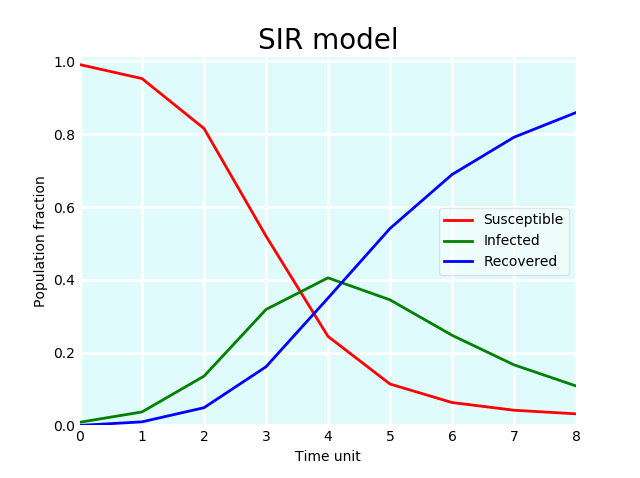
\includegraphics[scale=0.8]{Images/Figure_1.png}
\end{center}

\subsection{Bài toán 3}	
Để tìm ra các giá trị $\beta$ và $\gamma$, ta bắt đầu ước lượng $\beta_0$ và $\gamma_0$ bằng giá trị dương của phân phối chuẩn với trung bình là 0 và độ lệch chuẩn 0.3. Giả sử chúng ta tính  100 cặp giá trị $\beta$ và $\gamma$. Ta sử dụng phương pháp Metropolis-Hastings để tính các giá trị này và được đồ thị sau.
\begin{center}
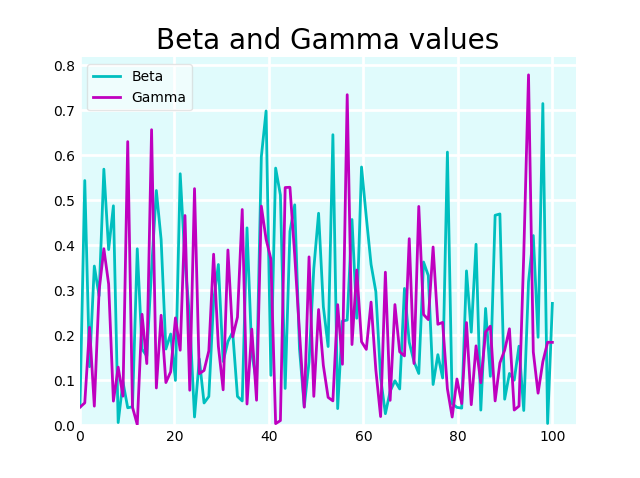
\includegraphics[scale=0.8]{Images/Figure_2.png}
\end{center}
\subsection{Bài toán 4}
Chúng ta sẽ lấy dữ liệu của khu vực Mỹ để ước lượng giá trị $R_0$. Thư viện pandas của python sẽ giúp ta lấy dữ liệu từ \url{https://raw.githubusercontent.com/CSSEGISandData/COVID-19/master/archived_data/archived_time_series/time_series_19-covid-Confirmed_archived_0325.csv} và \url{https://raw.githubusercontent.com/CSSEGISandData/COVID-19/master/archived_data/archived_time_series/time_series_19-covid-Confirmed_archived_0325.csv}. \\
Các dữ liệu Infected và Recovered của từng ngày sẽ được lưu vào hai mảng lI và LR tương ứng. Sử dụng công thức $(20)$ trong đề bài cùng với số lượng mẫu $\beta$ và $\gamma$ là 100, chúng ta tính các giá trị $R_0$ từ ngày $22/01/20$ đến $23/03/20$ của nước Mỹ. Do trong khoảng thời gian dịch chưa bùng phát mạnh nên các giá trị $\pi(X|\beta,\gamma)$ vô định.

\section{Kết luận}
	...


%%%%%%%%%%%%%%%%%%%%%%%%%%%%%%%%%
\addcontentsline{toc}{section}{Tài liệu}
\begin{thebibliography}{99999}
\bibitem[Dal]{Dal}{Dalgaard, P.} {\em Introductory Statistics with R.}  Springer 2008.

\bibitem[K-Z]{K-Z}{Kenett, R. S. and Zacks, S.}
{\em Modern Industrial Statistics: with applications in R, MINITAB and JMP,} 2nd ed.,  John Wiley and Sons, 2014.

\bibitem[Ker]{Ker}{Kerns, G. J.}
{\em Introduction to Probability and Statistics Using R,} 2nd ed., CRC 2015.

\end{thebibliography}
\end{document}

